\documentclass[]{article}
\usepackage{lmodern}
\usepackage{amssymb,amsmath}
\usepackage{ifxetex,ifluatex}
\usepackage{fixltx2e} % provides \textsubscript
\ifnum 0\ifxetex 1\fi\ifluatex 1\fi=0 % if pdftex
  \usepackage[T1]{fontenc}
  \usepackage[utf8]{inputenc}
\else % if luatex or xelatex
  \ifxetex
    \usepackage{mathspec}
  \else
    \usepackage{fontspec}
  \fi
  \defaultfontfeatures{Ligatures=TeX,Scale=MatchLowercase}
\fi
% use upquote if available, for straight quotes in verbatim environments
\IfFileExists{upquote.sty}{\usepackage{upquote}}{}
% use microtype if available
\IfFileExists{microtype.sty}{%
\usepackage{microtype}
\UseMicrotypeSet[protrusion]{basicmath} % disable protrusion for tt fonts
}{}
\usepackage[margin=1in]{geometry}
\usepackage{hyperref}
\hypersetup{unicode=true,
            pdftitle={Rbeginner: R and RStudio -- a first tour},
            pdfauthor={Mette Langaas and Martina Hall, Department of Mathematical Sciences, NTNU},
            pdfborder={0 0 0},
            breaklinks=true}
\urlstyle{same}  % don't use monospace font for urls
\usepackage{color}
\usepackage{fancyvrb}
\newcommand{\VerbBar}{|}
\newcommand{\VERB}{\Verb[commandchars=\\\{\}]}
\DefineVerbatimEnvironment{Highlighting}{Verbatim}{commandchars=\\\{\}}
% Add ',fontsize=\small' for more characters per line
\usepackage{framed}
\definecolor{shadecolor}{RGB}{248,248,248}
\newenvironment{Shaded}{\begin{snugshade}}{\end{snugshade}}
\newcommand{\KeywordTok}[1]{\textcolor[rgb]{0.13,0.29,0.53}{\textbf{#1}}}
\newcommand{\DataTypeTok}[1]{\textcolor[rgb]{0.13,0.29,0.53}{#1}}
\newcommand{\DecValTok}[1]{\textcolor[rgb]{0.00,0.00,0.81}{#1}}
\newcommand{\BaseNTok}[1]{\textcolor[rgb]{0.00,0.00,0.81}{#1}}
\newcommand{\FloatTok}[1]{\textcolor[rgb]{0.00,0.00,0.81}{#1}}
\newcommand{\ConstantTok}[1]{\textcolor[rgb]{0.00,0.00,0.00}{#1}}
\newcommand{\CharTok}[1]{\textcolor[rgb]{0.31,0.60,0.02}{#1}}
\newcommand{\SpecialCharTok}[1]{\textcolor[rgb]{0.00,0.00,0.00}{#1}}
\newcommand{\StringTok}[1]{\textcolor[rgb]{0.31,0.60,0.02}{#1}}
\newcommand{\VerbatimStringTok}[1]{\textcolor[rgb]{0.31,0.60,0.02}{#1}}
\newcommand{\SpecialStringTok}[1]{\textcolor[rgb]{0.31,0.60,0.02}{#1}}
\newcommand{\ImportTok}[1]{#1}
\newcommand{\CommentTok}[1]{\textcolor[rgb]{0.56,0.35,0.01}{\textit{#1}}}
\newcommand{\DocumentationTok}[1]{\textcolor[rgb]{0.56,0.35,0.01}{\textbf{\textit{#1}}}}
\newcommand{\AnnotationTok}[1]{\textcolor[rgb]{0.56,0.35,0.01}{\textbf{\textit{#1}}}}
\newcommand{\CommentVarTok}[1]{\textcolor[rgb]{0.56,0.35,0.01}{\textbf{\textit{#1}}}}
\newcommand{\OtherTok}[1]{\textcolor[rgb]{0.56,0.35,0.01}{#1}}
\newcommand{\FunctionTok}[1]{\textcolor[rgb]{0.00,0.00,0.00}{#1}}
\newcommand{\VariableTok}[1]{\textcolor[rgb]{0.00,0.00,0.00}{#1}}
\newcommand{\ControlFlowTok}[1]{\textcolor[rgb]{0.13,0.29,0.53}{\textbf{#1}}}
\newcommand{\OperatorTok}[1]{\textcolor[rgb]{0.81,0.36,0.00}{\textbf{#1}}}
\newcommand{\BuiltInTok}[1]{#1}
\newcommand{\ExtensionTok}[1]{#1}
\newcommand{\PreprocessorTok}[1]{\textcolor[rgb]{0.56,0.35,0.01}{\textit{#1}}}
\newcommand{\AttributeTok}[1]{\textcolor[rgb]{0.77,0.63,0.00}{#1}}
\newcommand{\RegionMarkerTok}[1]{#1}
\newcommand{\InformationTok}[1]{\textcolor[rgb]{0.56,0.35,0.01}{\textbf{\textit{#1}}}}
\newcommand{\WarningTok}[1]{\textcolor[rgb]{0.56,0.35,0.01}{\textbf{\textit{#1}}}}
\newcommand{\AlertTok}[1]{\textcolor[rgb]{0.94,0.16,0.16}{#1}}
\newcommand{\ErrorTok}[1]{\textcolor[rgb]{0.64,0.00,0.00}{\textbf{#1}}}
\newcommand{\NormalTok}[1]{#1}
\usepackage{longtable,booktabs}
\usepackage{graphicx,grffile}
\makeatletter
\def\maxwidth{\ifdim\Gin@nat@width>\linewidth\linewidth\else\Gin@nat@width\fi}
\def\maxheight{\ifdim\Gin@nat@height>\textheight\textheight\else\Gin@nat@height\fi}
\makeatother
% Scale images if necessary, so that they will not overflow the page
% margins by default, and it is still possible to overwrite the defaults
% using explicit options in \includegraphics[width, height, ...]{}
\setkeys{Gin}{width=\maxwidth,height=\maxheight,keepaspectratio}
\IfFileExists{parskip.sty}{%
\usepackage{parskip}
}{% else
\setlength{\parindent}{0pt}
\setlength{\parskip}{6pt plus 2pt minus 1pt}
}
\setlength{\emergencystretch}{3em}  % prevent overfull lines
\providecommand{\tightlist}{%
  \setlength{\itemsep}{0pt}\setlength{\parskip}{0pt}}
\setcounter{secnumdepth}{0}
% Redefines (sub)paragraphs to behave more like sections
\ifx\paragraph\undefined\else
\let\oldparagraph\paragraph
\renewcommand{\paragraph}[1]{\oldparagraph{#1}\mbox{}}
\fi
\ifx\subparagraph\undefined\else
\let\oldsubparagraph\subparagraph
\renewcommand{\subparagraph}[1]{\oldsubparagraph{#1}\mbox{}}
\fi

%%% Use protect on footnotes to avoid problems with footnotes in titles
\let\rmarkdownfootnote\footnote%
\def\footnote{\protect\rmarkdownfootnote}

%%% Change title format to be more compact
\usepackage{titling}

% Create subtitle command for use in maketitle
\newcommand{\subtitle}[1]{
  \posttitle{
    \begin{center}\large#1\end{center}
    }
}

\setlength{\droptitle}{-2em}

  \title{Rbeginner: R and RStudio -- a first tour}
    \pretitle{\vspace{\droptitle}\centering\huge}
  \posttitle{\par}
  \subtitle{TMA4268 Statistical Learning V2019. Module 1: INTRODUCTION TO
STATISTICAL LEARNING}
  \author{Mette Langaas and Martina Hall, Department of Mathematical Sciences,
NTNU}
    \preauthor{\centering\large\emph}
  \postauthor{\par}
      \predate{\centering\large\emph}
  \postdate{\par}
    \date{week 2, 2019}


\begin{document}
\maketitle

{
\setcounter{tocdepth}{2}
\tableofcontents
}
(Latest changes: 31.12.18: first version for 2019)

R is a free software environment for statistical computing and graphics.
It runs on a wide variety of UNIX platforms, Windows and MacOS. R can be
downloaded from \url{http://www.r-project.org/}.

We recommend that you run R using the RStudio IDE (integrated
development environment). RStudio can be downloaded from
\url{http://rstudio.org/}.\\
Notice: you need to download both R and RStudio.

If you need help on installing R and RStudio on you laptop computer,
contact \href{mailto:orakel@ntnu.no}{\nolinkurl{orakel@ntnu.no}}. If you
want to work at Nullrommet or Banachrommet at Matteland, R and RStudio
is already installed for you.

\section{Part A: Using RStudio - what are the different
windows?}\label{part-a-using-rstudio---what-are-the-different-windows}

Start RStudio. Then you (probably) have the following four windows.

\begin{itemize}
\tightlist
\item
  \textbf{Source} (aka script window) - upper left window: where you
  write your code and keep track of your work.
\item
  \textbf{Console} - lower left window: where the R commands are
  executed (so here is where you R installation lives). Sometimes also
  referred to as command window.\\
\item
  \textbf{Environment/History/Connections/Presentation} - upper right
  window: the objects that you have in your workspace, and the commands
  you have executed, and more.\\
\item
  \textbf{Files/Plots/Packages/Help/Viewer}- lower right: overview of
  your files, the plots you produce, the packages you have installed and
  loaded, and more.
\end{itemize}

\textbf{Source window}: (Make the source window active.) To start
writing a script press File- New File- R Script. To open an existing
file, press File- Open File- and select the file you want to open. The
file will open in the source window. To save this file, press File- Save
as- and go to the working directory there you want to put your TMA4268 R
files and save the file as ``name''.R (example: \texttt{myRintro.R}).
Files with R code usually have extension \texttt{.R}.

\textbf{Console window}: (Make the console window active.) To see your
working directory, you can write \texttt{getwd()}, and you will get your
location as output. You can also set your working directory to a certain
folder of choise by writing \texttt{setwd("location")} (Example:
\texttt{setwd("M:/Documents/TMA4268/")}). Now you are certain that all
your files will be put in this folder.

\textbf{Quitting}: It is always important to be able to quit a program:
when you are finished you may choose RStudio-Quit Rstudio (top menu
outside of the windows). Alternatively, you may write \texttt{q()}in the
console window to quit R (the parenthesis is because q is a function
that can have arguments to be given within the parentheses and you call
the function without any arguments). You will be asked if you want to
save your script and workspave. If you want to reuse your script later
(and of cause you want to do that - we aim at reproduciable research),
you should save it! If you answer yes to ``Save workspace image'' all
the objects you have created are found in a \texttt{.RData} file (more
about objects soon). This could be useful if you don't want to run all
the commands in the script again, because if you start R in the same
working directory all the objects you have created will be automatically
availble to you. More on objects next.

You can download the \textbf{RStudio IDE cheat sheet}:
\url{https://github.com/rstudio/cheatsheets/raw/master/rstudio-ide.pdf}

\section{Part B: Trying out
R-commands}\label{part-b-trying-out-r-commands}

To exceute your commands, you can either type directly in the console or
run the commands from the source window. In the \textbf{source window},
you can run the current line by pressing Ctrl and Enter (Windows) or CMD
and Enter (MacOS), or you can run select lines by marking them and
pressing Ctrl + Enter. You can also use the Run-button in the top right
corner of the window to run selected lines or commands, and the
Source-button in the top right corner to run everything in your Source
window.

\textbf{Q}: Write and execute the following commands. What have you done
mathematically here?

\begin{Shaded}
\begin{Highlighting}[]
\DecValTok{2} \OperatorTok{+}\StringTok{ }\DecValTok{3}
\DecValTok{2} \OperatorTok{*}\StringTok{ }\DecValTok{6}
\DecValTok{3} \OperatorTok{*}\StringTok{ }\DecValTok{10}\OperatorTok{^}\DecValTok{4} \OperatorTok{-}\StringTok{ }\DecValTok{3} \OperatorTok{*}\StringTok{ }\DecValTok{5}\OperatorTok{^}\DecValTok{2}
\DecValTok{10}\OperatorTok{^}\DecValTok{2} \OperatorTok{-}\StringTok{ }\DecValTok{1}
\DecValTok{10}\OperatorTok{^}\NormalTok{(}\DecValTok{2} \OperatorTok{-}\StringTok{ }\DecValTok{1}\NormalTok{)}
\KeywordTok{sqrt}\NormalTok{(}\DecValTok{9}\NormalTok{)}
\KeywordTok{log}\NormalTok{(}\DecValTok{3}\NormalTok{, }\DataTypeTok{base =} \DecValTok{10}\NormalTok{)}
\StringTok{`}\DataTypeTok{?}\StringTok{`}\NormalTok{(log)}
\NormalTok{log}
\KeywordTok{log10}\NormalTok{(}\DecValTok{3}\NormalTok{)}
\KeywordTok{log}\NormalTok{(}\DecValTok{3}\NormalTok{)}
\KeywordTok{exp}\NormalTok{(}\DecValTok{34}\NormalTok{)}
\KeywordTok{gamma}\NormalTok{(}\DecValTok{3}\NormalTok{)}
\KeywordTok{factorial}\NormalTok{(}\DecValTok{5}\NormalTok{)}
\KeywordTok{choose}\NormalTok{(}\DecValTok{10}\NormalTok{, }\DecValTok{4}\NormalTok{)}
\DecValTok{1}\OperatorTok{:}\DecValTok{4}
\KeywordTok{c}\NormalTok{(}\DecValTok{1}\NormalTok{, }\DecValTok{2}\NormalTok{, }\DecValTok{3}\NormalTok{, }\DecValTok{4}\NormalTok{)}
\KeywordTok{seq}\NormalTok{(}\DataTypeTok{from =} \DecValTok{1}\NormalTok{, }\DataTypeTok{to =} \DecValTok{4}\NormalTok{, }\DataTypeTok{by =} \DecValTok{1}\NormalTok{)}
\KeywordTok{sum}\NormalTok{(}\DecValTok{1}\OperatorTok{:}\DecValTok{5}\NormalTok{)}
\KeywordTok{prod}\NormalTok{(}\DecValTok{1}\OperatorTok{:}\DecValTok{5}\NormalTok{)}
\NormalTok{heights =}\StringTok{ }\KeywordTok{c}\NormalTok{(}\DecValTok{192}\NormalTok{, }\DecValTok{185}\NormalTok{, }\DecValTok{174}\NormalTok{, }\DecValTok{195}\NormalTok{, }\DecValTok{173}\NormalTok{)}
\NormalTok{shoes =}\StringTok{ }\KeywordTok{c}\NormalTok{(}\DecValTok{46}\NormalTok{, }\DecValTok{43}\NormalTok{, }\DecValTok{40}\NormalTok{, }\DecValTok{45}\NormalTok{, }\DecValTok{40}\NormalTok{)}
\NormalTok{ratio <-}\StringTok{ }\NormalTok{heights}\OperatorTok{/}\NormalTok{shoes}
\NormalTok{ratio}
\end{Highlighting}
\end{Shaded}

Here we have created three objects: \texttt{heights}, \texttt{shoes} and
\texttt{ratio}. Observe: we can both use \texttt{=} and
\texttt{\textless{}-} for assigning content to an object. Notice now
that the objects you assigned values to
(\texttt{heights,\ shows,\ ratio}) appear in the Enviroment window
(sorted as Data, Values or Functions, but you should only have Values so
far).

The function \texttt{c} combines values into a vector (concatenate).
Also, all the commands you have run are reported in the History window.

If you want to add comments, you do that by starting with a hashtag
symbol:

\begin{Shaded}
\begin{Highlighting}[]
\CommentTok{# now we quit}
\KeywordTok{q}\NormalTok{()}
\end{Highlighting}
\end{Shaded}

Save your work as \texttt{myRintro.R} - and we will try to open that in
Part C.

\section{Part C: Importing and
exporting}\label{part-c-importing-and-exporting}

\subsection{\texorpdfstring{Executing the commands in an R-file with
\texttt{source}}{Executing the commands in an R-file with source}}\label{executing-the-commands-in-an-r-file-with-source}

You ended Part B by quitting RStudio, now open RStudio again, and open
the file \texttt{myRintro.R} in your source window. Then either write:

\begin{Shaded}
\begin{Highlighting}[]
\KeywordTok{source}\NormalTok{(}\StringTok{"myRintro.R"}\NormalTok{)  }\CommentTok{#given that your working directory is wher myRintro.R is saved}
\end{Highlighting}
\end{Shaded}

or source with the source button in the upper right corner of the source
window.

It is also possible to source a file from the internet, for example a
version of Part B can be sources from the TMA4268 catalog:

\begin{Shaded}
\begin{Highlighting}[]
\KeywordTok{source}\NormalTok{(}\StringTok{"https://www.math.ntnu.no/emner/TMA4268/2019v/1Intro/RintroPartB.R"}\NormalTok{, }
    \DataTypeTok{echo =} \OtherTok{TRUE}\NormalTok{)}
\end{Highlighting}
\end{Shaded}

Here \texttt{echo=TRUE} echoes the commands being run- in addition to
the results of the commands.

Reading and writing data into R may be a bit tricky if the format of the
data is not defined exactly, so here we just show how to read three nice
formats.

You may also choose Enviroment (window upper right) -Import Data set -
and get help.

\subsection{Printing to and reading from a
csv-file}\label{printing-to-and-reading-from-a-csv-file}

\textbf{Q}: Study the R script below and find out what is done in each
line of the script.

\begin{Shaded}
\begin{Highlighting}[]
\NormalTok{n =}\StringTok{ }\DecValTok{1000}
\NormalTok{ds =}\StringTok{ }\KeywordTok{matrix}\NormalTok{(}\KeywordTok{rnorm}\NormalTok{(n), }\DataTypeTok{ncol =} \DecValTok{10}\NormalTok{)}
\KeywordTok{colnames}\NormalTok{(ds) =}\StringTok{ }\KeywordTok{paste}\NormalTok{(}\StringTok{"Variable"}\NormalTok{, }\DecValTok{1}\OperatorTok{:}\DecValTok{10}\NormalTok{, }\DataTypeTok{sep =} \StringTok{""}\NormalTok{)}
\KeywordTok{write.csv}\NormalTok{(ds, }\DataTypeTok{file =} \StringTok{"stnorm.csv"}\NormalTok{, }\DataTypeTok{row.names =} \OtherTok{FALSE}\NormalTok{)  }\CommentTok{#do not want 1:100 as rownames}
\KeywordTok{getwd}\NormalTok{()}
\KeywordTok{list.files}\NormalTok{()  }\CommentTok{#files in the folder of getwd()}
\NormalTok{dss =}\StringTok{ }\KeywordTok{read.csv}\NormalTok{(}\DataTypeTok{file =} \StringTok{"stnorm.csv"}\NormalTok{, }\DataTypeTok{header =} \OtherTok{TRUE}\NormalTok{)}
\KeywordTok{dim}\NormalTok{(dss)}
\KeywordTok{typeof}\NormalTok{(dss)}
\KeywordTok{head}\NormalTok{(dss)}
\end{Highlighting}
\end{Shaded}

\subsection{Printing to and reading from other file
formats}\label{printing-to-and-reading-from-other-file-formats}

There exists may packages to read different type of input data, and
reading \texttt{xls} files can be done using the package
\texttt{readxl}.

\subsection{Exporting plots}\label{exporting-plots}

We will talk more about generating random data from different
distribution in \texttt{Rintermediate.R} and more about plotting in Part
F. However, the following commands draws 100 realizations from the
standard normal distribution and makes a boxplot. Write these commands
and run them.

\begin{Shaded}
\begin{Highlighting}[]
\NormalTok{ds =}\StringTok{ }\KeywordTok{rnorm}\NormalTok{(}\DecValTok{100}\NormalTok{)}
\KeywordTok{boxplot}\NormalTok{(ds)}
\end{Highlighting}
\end{Shaded}

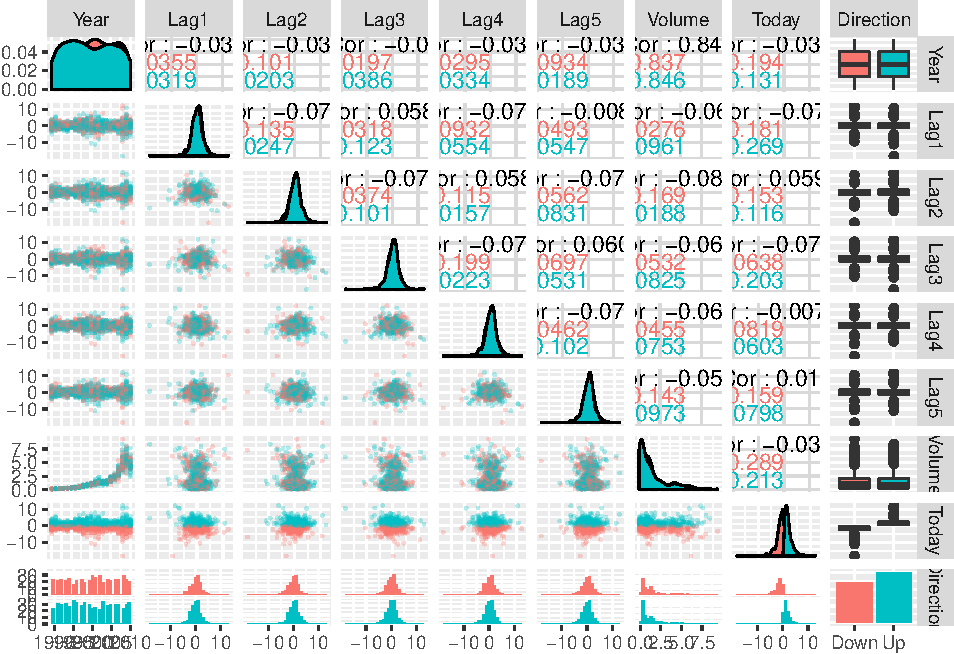
\includegraphics{Rbeginner_files/figure-latex/unnamed-chunk-6-1.pdf}

You how should have a boxplot in your Plots window - looking similar to
the one shown here. \textbf{Q}: What are the different parts of this
boxplot? Hint: median, 1 and 3rd quantiles. To read what the function
\texttt{boxplot} does you may write \texttt{help(boxplot)} or just
\texttt{?boxplot}. How are the whiskers defined?

Now, we want to export this plot - maybe to be put on a webpage or just
for fun (we will use R Markdown for our compulsory exercises and will
then not need to export plots).

You may save the plot (for example as pdf or svg) Export in the Plots
window, or alternatively you may write

\begin{Shaded}
\begin{Highlighting}[]
\KeywordTok{dev.copy2pdf}\NormalTok{(}\DataTypeTok{file =} \StringTok{"box.pdf"}\NormalTok{)}
\end{Highlighting}
\end{Shaded}

The will produce a pdf-file thtat is saved to your working directory.

A third solution \texttt{pdf("box.pdf");\ boxplot(ds);\ dev.off()}to
make a file named box.pdf with the boxplot, then it is possible to save
many plots together in one pdf-file - just add more plots before closing
the pdf-file with \texttt{dev.off()}.

\section{Part D: Packages - and
functions}\label{part-d-packages---and-functions}

R is a free and open source program. Everyone can contribute with making
functions (like \texttt{boxplot} and \texttt{rnorm}) and packages
(collection of functions and data sets), and there exists a \emph{lot}
of available packages. Some are already included in the default R
session, like the package \texttt{stats} that includes many basic
functions for doing statistics.

Every statistical researcher who would like to to get their new
statistitical methods used will make an R package and distribute it with
their article (on the new method). Most books also comes with R packages
with data sets and functions. Our ISL book has the package
\texttt{ISLR}, hosted on the most widely used service for R packages:
CRAN. See the official page for the package here:
\url{https://cran.r-project.org/web/packages/ISLR/index.html}.

To install an R package from CRAN you go to the Packages tab and see if
the packages is already available on your computer. If you see ISLR in
this list just press the square next to ISLR to load the package into R.

If you don't see ISLR you will have to download it from CRAN. Do this by
either pressing Install on the top left corner of the Packages window,
CRAN is already filled as ``Install from'' and then write ``ISLR'' as
the name of the package to install, and nice to have chosen ``install
dependencies'' (then packages that ISLR depend on will also be
installed). Then press ``Install''. You might have to select from
different mirrors for CRAN - choose Norway, and you are good to go. Then
``ISLR'' should pop up in the list of packages installed, and you tick
(in the square) to load the package into R.

Alternatively, in the console (or source) window you may write:

\begin{Shaded}
\begin{Highlighting}[]
\KeywordTok{install.packages}\NormalTok{(}\StringTok{"ISLR"}\NormalTok{)}
\KeywordTok{library}\NormalTok{(ISLR)  }\CommentTok{# to make the package available in the current session}
\end{Highlighting}
\end{Shaded}

Now the packages is installed and loaded to the current session.
Remember that whenever starting a new session, you need to reload the
packages you want to use, using the \texttt{library()} function, or
ticking the square next to ISLR in the Packages window.

\begin{Shaded}
\begin{Highlighting}[]
\KeywordTok{library}\NormalTok{(}\DataTypeTok{help =} \StringTok{"ISLR"}\NormalTok{)}
\end{Highlighting}
\end{Shaded}

\textbf{Q}: Look at the contents of the \texttt{ISLR} to see that only
data sets are available - you may also see that by selecting the name
ISLR in the Packages window. To know more about the data set named
\texttt{NCI60} either just select the data set in the Packages window,
or write \texttt{help(NCI60)} after ISLR is loaded. What can you say
about \texttt{NCI60}?

Another package that we will use is \texttt{car}. \textbf{Q}: Install
the \texttt{car} package from CRAN, check the content of the package
(data sets and functions) and investigate

We will be using a lot of packages in this course, and the ones we use
will be listed on the start of each module page. We would assume that
you have loaded these packages if you want to reproduce that statistical
analyses on the module pages.

Before start using the functions of the package, it is often a good idea
to visit the help pages of the package to see which functions and data
sets are available, how they are used, what they calculate, and the
output they give, etx.. These pages are found in the Help window to the
left or typing \texttt{?name}in the console, (ex. \texttt{?mean}).

In the stats package, you find functions for making and evaluating
distributions. We use the function \texttt{rnorm} to sample independent
data from the univariate normal distribution.

\begin{Shaded}
\begin{Highlighting}[]
\NormalTok{rnorm  }\CommentTok{#lists the function code}
\StringTok{`}\DataTypeTok{?}\StringTok{`}\NormalTok{(rnorm  }\CommentTok{#help pages for the function}
\NormalTok{)}
\KeywordTok{rnorm}\NormalTok{()  }\CommentTok{#gives error}
\KeywordTok{rnorm}\NormalTok{(}\DataTypeTok{n =} \DecValTok{100}\NormalTok{, }\DataTypeTok{mean =} \DecValTok{0}\NormalTok{, }\DataTypeTok{sd =} \DecValTok{1}\NormalTok{)  }\CommentTok{#draw random samples from this distribution}
\StringTok{`}\DataTypeTok{?}\StringTok{`}\NormalTok{(lm  }\CommentTok{# more to see, will be what we use to perform linear regression}
\NormalTok{)}
\end{Highlighting}
\end{Shaded}

\section{Part E: More on vectors and
matrices}\label{part-e-more-on-vectors-and-matrices}

R can handle both numeric and non numeric data. The concatenate
\texttt{c}-function can handle both numeric and non-numeric data, but be
careful when mixing them.

\textbf{Q}: Go through theses commands and see what is produced.

\begin{Shaded}
\begin{Highlighting}[]
\NormalTok{x =}\StringTok{ }\KeywordTok{c}\NormalTok{(}\DecValTok{1}\NormalTok{, }\DecValTok{2}\NormalTok{, }\DecValTok{3}\NormalTok{)}
\KeywordTok{typeof}\NormalTok{(x)}
\NormalTok{y =}\StringTok{ }\KeywordTok{c}\NormalTok{(}\StringTok{"a"}\NormalTok{, }\StringTok{"b"}\NormalTok{, }\StringTok{"c"}\NormalTok{)}
\KeywordTok{typeof}\NormalTok{(y)}

\NormalTok{u =}\StringTok{ }\KeywordTok{c}\NormalTok{(}\StringTok{"1"}\NormalTok{, }\StringTok{"2"}\NormalTok{, }\StringTok{"3"}\NormalTok{)}
\KeywordTok{typeof}\NormalTok{(u)}
\NormalTok{v =}\StringTok{ }\KeywordTok{as.numeric}\NormalTok{(u)}
\KeywordTok{typeof}\NormalTok{(v)}

\NormalTok{z =}\StringTok{ }\KeywordTok{c}\NormalTok{(}\StringTok{"red"}\NormalTok{, }\DecValTok{1}\NormalTok{, }\StringTok{"yellow"}\NormalTok{, }\DecValTok{2}\NormalTok{)}
\KeywordTok{typeof}\NormalTok{(z)}
\CommentTok{# w = z - 1 this gives error}
\end{Highlighting}
\end{Shaded}

\begin{verbatim}
## [1] "double"
## [1] "character"
## [1] "character"
## [1] "double"
## [1] "character"
\end{verbatim}

Logical operators are also available, \texttt{==} for equality,
\texttt{!=} for not equal to, \texttt{\textgreater{}=} for greater than
or equal to, etc.

\begin{Shaded}
\begin{Highlighting}[]
\NormalTok{gender =}\StringTok{ }\KeywordTok{factor}\NormalTok{(}\KeywordTok{c}\NormalTok{(}\StringTok{"male"}\NormalTok{, }\StringTok{"female"}\NormalTok{, }\StringTok{"female"}\NormalTok{, }\StringTok{"male"}\NormalTok{))}
\NormalTok{gender}
\KeywordTok{sum}\NormalTok{(gender }\OperatorTok{==}\StringTok{ "male"}\NormalTok{)}
\KeywordTok{table}\NormalTok{(gender)}
\end{Highlighting}
\end{Shaded}

\begin{verbatim}
## [1] male   female female male  
## Levels: female male
## [1] 2
## gender
## female   male 
##      2      2
\end{verbatim}

Useful for vectors:

\begin{Shaded}
\begin{Highlighting}[]
\NormalTok{x =}\StringTok{ }\DecValTok{1}\OperatorTok{:}\DecValTok{5}
\NormalTok{x =}\StringTok{ }\KeywordTok{seq}\NormalTok{(}\DecValTok{1}\NormalTok{, }\DecValTok{5}\NormalTok{, }\DataTypeTok{length =} \DecValTok{5}\NormalTok{)}
\NormalTok{x =}\StringTok{ }\KeywordTok{c}\NormalTok{(}\DecValTok{1}\NormalTok{, }\DecValTok{2}\NormalTok{, }\DecValTok{3}\NormalTok{, }\DecValTok{4}\NormalTok{, }\DecValTok{5}\NormalTok{)}
\DecValTok{2} \OperatorTok\StringTok{ }\NormalTok{x}
\DecValTok{6} \OperatorTok\StringTok{ }\NormalTok{x}
\NormalTok{x[}\DecValTok{2}\NormalTok{] =}\StringTok{ }\DecValTok{10}
\NormalTok{x[}\DecValTok{3}\OperatorTok{:}\DecValTok{4}\NormalTok{] =}\StringTok{ }\DecValTok{0}
\NormalTok{x[}\OperatorTok{-}\DecValTok{2}\NormalTok{] =}\StringTok{ }\DecValTok{1}
\NormalTok{x[}\KeywordTok{c}\NormalTok{(}\DecValTok{1}\NormalTok{, }\DecValTok{4}\NormalTok{)] =}\StringTok{ }\DecValTok{4}
\NormalTok{x[x }\OperatorTok{>}\StringTok{ }\DecValTok{4}\NormalTok{] =}\StringTok{ }\DecValTok{10}
\NormalTok{y =}\StringTok{ }\KeywordTok{log}\NormalTok{(x)}
\NormalTok{z =}\StringTok{ }\KeywordTok{exp}\NormalTok{(y)}
\NormalTok{z =}\StringTok{ }\NormalTok{z }\OperatorTok{+}\StringTok{ }\NormalTok{y}
\NormalTok{y =}\StringTok{ }\NormalTok{x }\OperatorTok{*}\StringTok{ }\NormalTok{y}
\NormalTok{z =}\StringTok{ }\NormalTok{y}\OperatorTok{/}\NormalTok{x}
\NormalTok{a =}\StringTok{ }\KeywordTok{t}\NormalTok{(x) }\OperatorTok\StringTok{ }\NormalTok{y  }\CommentTok{# t(): transpose}
\KeywordTok{min}\NormalTok{(x)}
\KeywordTok{max}\NormalTok{(x)}
\KeywordTok{sum}\NormalTok{(x)}
\KeywordTok{mean}\NormalTok{(x)}
\KeywordTok{var}\NormalTok{(x)}
\KeywordTok{length}\NormalTok{(x)}
\KeywordTok{sort}\NormalTok{(x)}
\KeywordTok{order}\NormalTok{(x)}
\KeywordTok{sort}\NormalTok{(x) }\OperatorTok{==}\StringTok{ }\NormalTok{x[}\KeywordTok{order}\NormalTok{(x)]}
\end{Highlighting}
\end{Shaded}

Notice the length of your vectors when doing calculations with two
vectors.

\begin{Shaded}
\begin{Highlighting}[]
\NormalTok{x =}\StringTok{ }\DecValTok{1}\OperatorTok{:}\DecValTok{5}
\NormalTok{y =}\StringTok{ }\DecValTok{2}
\NormalTok{x }\OperatorTok{-}\StringTok{ }\NormalTok{y}
\DecValTok{5} \OperatorTok{*}\StringTok{ }\NormalTok{x}

\NormalTok{z =}\StringTok{ }\DecValTok{10}\OperatorTok{:}\DecValTok{15}
\NormalTok{w =}\StringTok{ }\DecValTok{1}\OperatorTok{:}\DecValTok{2}
\NormalTok{z }\OperatorTok{-}\StringTok{ }\NormalTok{w}
\end{Highlighting}
\end{Shaded}

\begin{verbatim}
## [1] -1  0  1  2  3
## [1]  5 10 15 20 25
## [1]  9  9 11 11 13 13
\end{verbatim}

What happens here?

For matrices:

\begin{Shaded}
\begin{Highlighting}[]
\NormalTok{A =}\StringTok{ }\KeywordTok{matrix}\NormalTok{(}\DecValTok{1}\OperatorTok{:}\DecValTok{6}\NormalTok{, }\DataTypeTok{nrow =} \DecValTok{3}\NormalTok{, }\DataTypeTok{ncol =} \DecValTok{2}\NormalTok{)}
\NormalTok{A}
\end{Highlighting}
\end{Shaded}

\begin{verbatim}
##      [,1] [,2]
## [1,]    1    4
## [2,]    2    5
## [3,]    3    6
\end{verbatim}

\begin{Shaded}
\begin{Highlighting}[]
\NormalTok{B =}\StringTok{ }\KeywordTok{matrix}\NormalTok{(}\DecValTok{1}\OperatorTok{:}\DecValTok{6}\NormalTok{, }\DataTypeTok{nrow =} \DecValTok{2}\NormalTok{, }\DataTypeTok{ncol =} \DecValTok{3}\NormalTok{, }\DataTypeTok{byrow =} \OtherTok{TRUE}\NormalTok{)}
\NormalTok{B}
\end{Highlighting}
\end{Shaded}

\begin{verbatim}
##      [,1] [,2] [,3]
## [1,]    1    2    3
## [2,]    4    5    6
\end{verbatim}

\begin{Shaded}
\begin{Highlighting}[]
\NormalTok{A }\OperatorTok\StringTok{ }\NormalTok{B  }\CommentTok{# matrix multiplication}
\NormalTok{A }\OperatorTok{*}\StringTok{ }\KeywordTok{t}\NormalTok{(B)}
\NormalTok{A }\OperatorTok\StringTok{ }\KeywordTok{t}\NormalTok{(A)}
\NormalTok{A}\OperatorTok{^}\DecValTok{2}
\end{Highlighting}
\end{Shaded}

\begin{verbatim}
##      [,1] [,2] [,3]
## [1,]   17   22   27
## [2,]   22   29   36
## [3,]   27   36   45
##      [,1] [,2]
## [1,]    1   16
## [2,]    4   25
## [3,]    9   36
##      [,1] [,2] [,3]
## [1,]   17   22   27
## [2,]   22   29   36
## [3,]   27   36   45
##      [,1] [,2]
## [1,]    1   16
## [2,]    4   25
## [3,]    9   36
\end{verbatim}

The functions \texttt{cbind} (column bind) and \texttt{rbind} (row bind)
can also be used to create matrices:

\begin{Shaded}
\begin{Highlighting}[]
\NormalTok{x1 =}\StringTok{ }\DecValTok{1}\OperatorTok{:}\DecValTok{3}
\NormalTok{x2 =}\StringTok{ }\KeywordTok{c}\NormalTok{(}\DecValTok{7}\NormalTok{, }\DecValTok{6}\NormalTok{, }\DecValTok{6}\NormalTok{)}
\NormalTok{x3 =}\StringTok{ }\KeywordTok{c}\NormalTok{(}\DecValTok{12}\NormalTok{, }\DecValTok{19}\NormalTok{, }\DecValTok{21}\NormalTok{)}
\NormalTok{A =}\StringTok{ }\KeywordTok{cbind}\NormalTok{(x1, x2, x3)  }\CommentTok{# Bind vectors x1, x2, and x3 into a matrix.}
\CommentTok{# Treats each as a column.}
\NormalTok{A =}\StringTok{ }\KeywordTok{rbind}\NormalTok{(x1, x2, x3)  }\CommentTok{# Bind vectors x1, x2, and x3 into a matrix.}
\CommentTok{# Treats each as a row.}
\end{Highlighting}
\end{Shaded}

Other matrix commands are

\begin{Shaded}
\begin{Highlighting}[]
\KeywordTok{dim}\NormalTok{(A)  }\CommentTok{# get the dimensions of a matrix}
\KeywordTok{nrow}\NormalTok{(A)  }\CommentTok{# number of rows}
\KeywordTok{ncol}\NormalTok{(A)  }\CommentTok{# number of columns}
\KeywordTok{apply}\NormalTok{(A, }\DecValTok{1}\NormalTok{, sum)  }\CommentTok{# apply the sum function to the rows of A}
\KeywordTok{apply}\NormalTok{(A, }\DecValTok{2}\NormalTok{, sum)  }\CommentTok{# apply the sum function to the columns of A}
\KeywordTok{sum}\NormalTok{(}\KeywordTok{diag}\NormalTok{(A))  }\CommentTok{# trace of A}
\NormalTok{A =}\StringTok{ }\KeywordTok{diag}\NormalTok{(}\DecValTok{1}\OperatorTok{:}\DecValTok{3}\NormalTok{)}
\KeywordTok{solve}\NormalTok{(A)  }\CommentTok{# inverse of A, in general solve(A,b) solves Ax=b wrt x}
\KeywordTok{det}\NormalTok{(A)  }\CommentTok{# determinant of A}
\end{Highlighting}
\end{Shaded}

\section{Part F: Plotting}\label{part-f-plotting}

Create a plot

\begin{Shaded}
\begin{Highlighting}[]
\NormalTok{x <-}\StringTok{ }\KeywordTok{seq}\NormalTok{(}\OperatorTok{-}\DecValTok{4}\NormalTok{, }\DecValTok{4}\NormalTok{, }\DataTypeTok{length =} \DecValTok{500}\NormalTok{)}
\NormalTok{y <-}\StringTok{ }\NormalTok{x}\OperatorTok{^}\DecValTok{2} \OperatorTok{-}\StringTok{ }\DecValTok{1}
\KeywordTok{plot}\NormalTok{(x, y, }\DataTypeTok{type =} \StringTok{"l"}\NormalTok{, }\DataTypeTok{main =} \StringTok{"My plot"}\NormalTok{, }\DataTypeTok{xlab =} \StringTok{"x"}\NormalTok{, }\DataTypeTok{ylab =} \StringTok{"y"}\NormalTok{)}
\KeywordTok{abline}\NormalTok{(}\DataTypeTok{v =} \DecValTok{3}\NormalTok{)}
\KeywordTok{abline}\NormalTok{(}\DataTypeTok{h =} \DecValTok{5}\NormalTok{)}
\end{Highlighting}
\end{Shaded}

\includegraphics{Rbeginner_files/figure-latex/unnamed-chunk-20-1.pdf}

To draw the plot in the way you want, check the help pages of the plot
function to see which input values you can change to make your plot look
the way you want to.

The package \texttt{ggplot2}is a powerful tool for making nice plots. In
this package, the function \texttt{qplot()}can be used to compute the
basic graphics from the plot function - however it is better to use the
grammar of graphics that is the core of the \texttt{ggplot2} package -
if you want to learn more about the grammar of graphics you should start
by reading \href{http://r4ds.had.co.nz/data-visualisation.html}{Chapter
3 of the book \texttt{R\ for\ Data\ Science}}.

Before diving in to this, the list below shows some basic tools for
plotting using both \texttt{plot()}and \texttt{qplot()} (the last from
the \texttt{ggplot2} package).

\begin{longtable}[]{@{}lll@{}}
\toprule
\begin{minipage}[b]{0.41\columnwidth}\raggedright\strut
Description\strut
\end{minipage} & \begin{minipage}[b]{0.25\columnwidth}\raggedright\strut
Base Graphics\strut
\end{minipage} & \begin{minipage}[b]{0.25\columnwidth}\raggedright\strut
ggplot2\strut
\end{minipage}\tabularnewline
\midrule
\endhead
\begin{minipage}[t]{0.41\columnwidth}\raggedright\strut
Plot y versus x using points\strut
\end{minipage} & \begin{minipage}[t]{0.25\columnwidth}\raggedright\strut
plot(x, y)\strut
\end{minipage} & \begin{minipage}[t]{0.25\columnwidth}\raggedright\strut
qplot(x, y)\strut
\end{minipage}\tabularnewline
\begin{minipage}[t]{0.41\columnwidth}\raggedright\strut
Plot y versus x using lines\strut
\end{minipage} & \begin{minipage}[t]{0.25\columnwidth}\raggedright\strut
plot(x, y, type = ``l'')\strut
\end{minipage} & \begin{minipage}[t]{0.25\columnwidth}\raggedright\strut
qplot(x, y, geom = ``line'')\strut
\end{minipage}\tabularnewline
\begin{minipage}[t]{0.41\columnwidth}\raggedright\strut
Plot y versus x using both points and lines\strut
\end{minipage} & \begin{minipage}[t]{0.25\columnwidth}\raggedright\strut
plot(x, y, type = ``b'')\strut
\end{minipage} & \begin{minipage}[t]{0.25\columnwidth}\raggedright\strut
qplot(x, y, geom = c(``point'', ``line''))\strut
\end{minipage}\tabularnewline
\begin{minipage}[t]{0.41\columnwidth}\raggedright\strut
Boxplot of x\strut
\end{minipage} & \begin{minipage}[t]{0.25\columnwidth}\raggedright\strut
boxplot(x)\strut
\end{minipage} & \begin{minipage}[t]{0.25\columnwidth}\raggedright\strut
qplot(x, geom = ``boxplot'')\strut
\end{minipage}\tabularnewline
\begin{minipage}[t]{0.41\columnwidth}\raggedright\strut
Side-by-side boxplot of x and y\strut
\end{minipage} & \begin{minipage}[t]{0.25\columnwidth}\raggedright\strut
boxplot(x, y)\strut
\end{minipage} & \begin{minipage}[t]{0.25\columnwidth}\raggedright\strut
qplot(x, y, geom = ``boxplot'')\strut
\end{minipage}\tabularnewline
\begin{minipage}[t]{0.41\columnwidth}\raggedright\strut
Histogram of x\strut
\end{minipage} & \begin{minipage}[t]{0.25\columnwidth}\raggedright\strut
hist(x)\strut
\end{minipage} & \begin{minipage}[t]{0.25\columnwidth}\raggedright\strut
qplot(x, geom = ``histogram'')\strut
\end{minipage}\tabularnewline
\bottomrule
\end{longtable}

Plotting will be an important part of any statistical analysis course.

\section{Part G: Writing a simple
function}\label{part-g-writing-a-simple-function}

When starting a function, you should start with the name of the function
and state if the function takes input values. Then you write the
function code inside the branches \({}\). Remember to return the output
of the function using \texttt{return()}.

\begin{Shaded}
\begin{Highlighting}[]
\NormalTok{myfunction <-}\StringTok{ }\ControlFlowTok{function}\NormalTok{(x, y) }\CommentTok{# myfunction is the name, x and y are the names of the inputs}
\NormalTok{\{}
\NormalTok{    n <-}\StringTok{ }\KeywordTok{c}\NormalTok{(}\KeywordTok{length}\NormalTok{(x), }\KeywordTok{length}\NormalTok{(y))}
\NormalTok{    m <-}\StringTok{ }\KeywordTok{c}\NormalTok{(}\KeywordTok{sum}\NormalTok{(x), }\KeywordTok{sum}\NormalTok{(y))}
\NormalTok{    p <-}\StringTok{ }\NormalTok{m}\OperatorTok{/}\NormalTok{n}
    \KeywordTok{return}\NormalTok{(p)}
\NormalTok{\}}
\end{Highlighting}
\end{Shaded}

\textbf{Q}: If \texttt{x} and \texttt{y} are two vectors of different
lengths - what does then the function return?

To start using the function, you must first run it through the console
so that it is in your enviroment (mark and run). Then you call the
function name and give your inputs like this.

\begin{Shaded}
\begin{Highlighting}[]
\NormalTok{a =}\StringTok{ }\DecValTok{1}\OperatorTok{:}\DecValTok{10}
\NormalTok{b =}\StringTok{ }\KeywordTok{seq}\NormalTok{(}\DataTypeTok{from =} \FloatTok{0.1}\NormalTok{, }\DataTypeTok{to =} \DecValTok{1}\NormalTok{, }\DataTypeTok{length =} \DecValTok{10}\NormalTok{)}
\NormalTok{p =}\StringTok{ }\KeywordTok{myfunction}\NormalTok{(}\DataTypeTok{x =}\NormalTok{ a, }\DataTypeTok{y =}\NormalTok{ b)  }\CommentTok{#assign output to a variable p}
\NormalTok{p}
\end{Highlighting}
\end{Shaded}

\begin{verbatim}
## [1] 5.50 0.55
\end{verbatim}

You can also use \texttt{if/else} sentences, \texttt{for/while}-loops
and \texttt{print()}.

\begin{Shaded}
\begin{Highlighting}[]
\NormalTok{lett =}\StringTok{ }\KeywordTok{c}\NormalTok{(}\StringTok{"a"}\NormalTok{, }\StringTok{"b"}\NormalTok{, }\StringTok{"c"}\NormalTok{, }\StringTok{"d"}\NormalTok{, }\StringTok{"e"}\NormalTok{, }\StringTok{"f"}\NormalTok{, }\StringTok{"g"}\NormalTok{, }\StringTok{"h"}\NormalTok{)}
\ControlFlowTok{for}\NormalTok{ (i }\ControlFlowTok{in} \DecValTok{1}\OperatorTok{:}\KeywordTok{length}\NormalTok{(lett)) \{}
    \KeywordTok{print}\NormalTok{(}\StringTok{"Now we work with:"}\NormalTok{)}
    \KeywordTok{print}\NormalTok{(lett[i])}
    \ControlFlowTok{if}\NormalTok{ (lett[i] }\OperatorTok{==}\StringTok{ "b"}\NormalTok{) \{}
        \KeywordTok{print}\NormalTok{(lett[i])}
\NormalTok{    \} }\ControlFlowTok{else}\NormalTok{ \{}
        \ControlFlowTok{if}\NormalTok{ (lett[i] }\OperatorTok{==}\StringTok{ "d"}\NormalTok{) \{}
            \KeywordTok{print}\NormalTok{(lett[i])}
\NormalTok{        \} }\ControlFlowTok{else}\NormalTok{ \{}
            \KeywordTok{print}\NormalTok{(}\StringTok{"not b or d"}\NormalTok{)}
\NormalTok{        \}}
\NormalTok{    \}}
\NormalTok{\}}
\end{Highlighting}
\end{Shaded}

While loopes can be written in a similar mannar, using \texttt{while}
instad of \texttt{for}.

\section{Part H: Lists and data
frames}\label{part-h-lists-and-data-frames}

Lists and data frames are good tools for storing and accessing your
data.

\subsection{Lists}\label{lists}

Using a list, there is no restrictions to the type of data you want to
store.

\begin{Shaded}
\begin{Highlighting}[]
\NormalTok{a =}\StringTok{ }\KeywordTok{c}\NormalTok{(}\StringTok{"male"}\NormalTok{, }\StringTok{"female"}\NormalTok{, }\StringTok{"male"}\NormalTok{, }\StringTok{"male"}\NormalTok{)}
\NormalTok{b =}\StringTok{ }\KeywordTok{matrix}\NormalTok{(}\KeywordTok{c}\NormalTok{(}\DecValTok{1}\OperatorTok{:}\DecValTok{6}\NormalTok{), }\DataTypeTok{ncol =} \DecValTok{2}\NormalTok{)}
\NormalTok{c =}\StringTok{ }\KeywordTok{rnorm}\NormalTok{(}\DecValTok{100}\NormalTok{, }\DataTypeTok{mean =} \DecValTok{0}\NormalTok{, }\DataTypeTok{sd =} \DecValTok{1}\NormalTok{)}
\NormalTok{my_list =}\StringTok{ }\KeywordTok{list}\NormalTok{(}\DataTypeTok{a =}\NormalTok{ a, }\DataTypeTok{b =}\NormalTok{ b, }\DataTypeTok{c =}\NormalTok{ c)}
\end{Highlighting}
\end{Shaded}

The list \texttt{my\_list} now consists of three objects, \texttt{a,\ b}
and \texttt{c}. To access the data in you list, you write

\begin{Shaded}
\begin{Highlighting}[]
\NormalTok{my_list[[}\DecValTok{1}\NormalTok{]]  }\CommentTok{#a}
\NormalTok{my_list[[}\DecValTok{2}\NormalTok{]]  }\CommentTok{#b}
\NormalTok{my_list[[}\DecValTok{3}\NormalTok{]]  }\CommentTok{#c}
\end{Highlighting}
\end{Shaded}

or

\begin{Shaded}
\begin{Highlighting}[]
\NormalTok{my_list}\OperatorTok{$}\NormalTok{a  }\CommentTok{#a}
\NormalTok{my_list}\OperatorTok{$}\NormalTok{b  }\CommentTok{#b}
\NormalTok{my_list}\OperatorTok{$}\NormalTok{c  }\CommentTok{#c}
\end{Highlighting}
\end{Shaded}

To access the second element in the object \texttt{a}, you write
\texttt{my\_list{[}{[}1{]}{]}{[}2{]}} or \texttt{my\_list\$a{[}2{]}}.

\subsection{Data frames}\label{data-frames}

When using a data frame, you need all your elements in the data frame to
be of equal length.

\begin{Shaded}
\begin{Highlighting}[]
\NormalTok{Sick =}\StringTok{ }\KeywordTok{c}\NormalTok{(}\DecValTok{0}\NormalTok{, }\DecValTok{1}\NormalTok{, }\DecValTok{1}\NormalTok{, }\DecValTok{0}\NormalTok{, }\DecValTok{0}\NormalTok{, }\DecValTok{0}\NormalTok{, }\DecValTok{1}\NormalTok{, }\DecValTok{0}\NormalTok{)}
\NormalTok{Age =}\StringTok{ }\KeywordTok{c}\NormalTok{(}\DecValTok{50}\NormalTok{, }\DecValTok{15}\NormalTok{, }\DecValTok{39}\NormalTok{, }\DecValTok{35}\NormalTok{, }\DecValTok{26}\NormalTok{, }\DecValTok{20}\NormalTok{, }\DecValTok{10}\NormalTok{, }\DecValTok{69}\NormalTok{)}
\NormalTok{Sex =}\StringTok{ }\KeywordTok{factor}\NormalTok{(}\KeywordTok{c}\NormalTok{(}\StringTok{"male"}\NormalTok{, }\StringTok{"female"}\NormalTok{, }\StringTok{"female"}\NormalTok{, }\StringTok{"male"}\NormalTok{, }\StringTok{"male"}\NormalTok{, }\StringTok{"male"}\NormalTok{, }\StringTok{"female"}\NormalTok{, }
    \StringTok{"male"}\NormalTok{))}
\NormalTok{df =}\StringTok{ }\KeywordTok{data.frame}\NormalTok{(}\DataTypeTok{Sick =}\NormalTok{ Sick, }\DataTypeTok{Age =}\NormalTok{ Age, }\DataTypeTok{Sex =}\NormalTok{ Sex)}
\end{Highlighting}
\end{Shaded}

To access the vectors in the data frame,

\begin{Shaded}
\begin{Highlighting}[]
\NormalTok{df}\OperatorTok{$}\NormalTok{Sick}
\NormalTok{df}\OperatorTok{$}\NormalTok{Age}
\NormalTok{df}\OperatorTok{$}\NormalTok{Sex}
\end{Highlighting}
\end{Shaded}

Similar to a list, we access elements in the data frame using
\texttt{df\$Sex{[}2{]}}. If your data frame is very large, it is easier
to view typing \texttt{View(df)}.

\section{What is next?}\label{what-is-next}

You may now move to
\href{https://www.math.ntnu.no/emner/TMA4268/2019v/1Intro/Rintermediate.html}{Rintermediate.html}
to see how R can be used on topics that should already be familiar to
you from TMA4240/TMA4245 Statistics - or similar courses. Or, if you did
ST1201 you can look at an overview of how the methods in ST1201 can be
performed in R:
\href{https://www.math.ntnu.no/emner/TMA4268/2019v/1Intro/ST1201inR.html}{ST1201inR.html}


\end{document}
